% !TEX encoding = UTF-8 Unicode
\documentclass{article}

\usepackage{polski}
\usepackage[utf8]{inputenc}
\usepackage{subfig}
\usepackage{multirow}
\usepackage{graphicx}

\usepackage[a4paper, left=2.5cm, right=2.5cm, top=3.5cm, bottom=3.5cm, headsep=1.2cm]{geometry}

\linespread{1.3}
\begin{document}
	
	\begin{titlepage}
		\centering
		{\scshape\LARGE Politechnika Wrocławska \par}
		{\scshape\Large Katedra Informatyki Technicznej\par}
		
		\vspace{1cm}
		{\scshape\Large Inżynieria Oprogramowania\par}
		\vspace{1.5cm}
		{\huge\bfseries \par}
		\vspace{2cm}
		{\Large\itshape Magdalena Biernat\par}
		{\Large\itshape Mateusz Bortkiewicz\par}
		\vfill
		Opiekun\par
		prof. dr hab. inż. Jan Magott 
		
		\vfill
		{\large \today\par}
	\end{titlepage}
	\newpage
	\section{Wprowadzenie}
	Sprawozdanie dotyczy trzynastych zajęć. Na tych laboratoriach pisaliśmy testy do swojego projektu. 
	
	\section{Cel laboratorium}
Nabycie umiejętności przygotowywania testów akceptacyjnych za pomocą narzędzia FitNesse.
\section{Laboratorium}
Wykonano testy dwóch klas.
\subsection{Testy w klasie TWypozyczenie}
Zawartość testów:
\begin{verbatim}
!define TEST_SYSTEM {slim}
!path C:\Users\magda\Desktop\Madzia\PWr\IO\repo_IO\Studia\Inżynieria oprogramowania\Testy
\Testy_fitnesse\build\classes
!|import|
|import java.text.DateFormat;|
|import java.text.ParseException;|
|import java.text.SimpleDateFormat;|
|import java.util.Date;|
|import klasy.TWypozyczenie;|
!|import|
|fitnesse|

!|testy_fitnesse.TestWypozyczenie|
|DataPoczatek|DataKoniec|dni?|
|2018-01-19|2018-01-24|5|
|2018-01-01|2018-01-11|10|
|2017-03-01|2017-03-13|12|
|2016-02-01|2016-02-09|8|
|2018-01-16|2018-01-19|3|
|2018-02-01|2018-02-17|16|
|2018-01-01|2018-01-13|12|
|2018-03-05|2018-03-06|1|
|2017-05-02|2017-05-11|9|
|2017-07-03|2017-08-04|32|
\end{verbatim}
\newpage
Efekt testów:
	\begin{figure}[!ht]
	\centering
	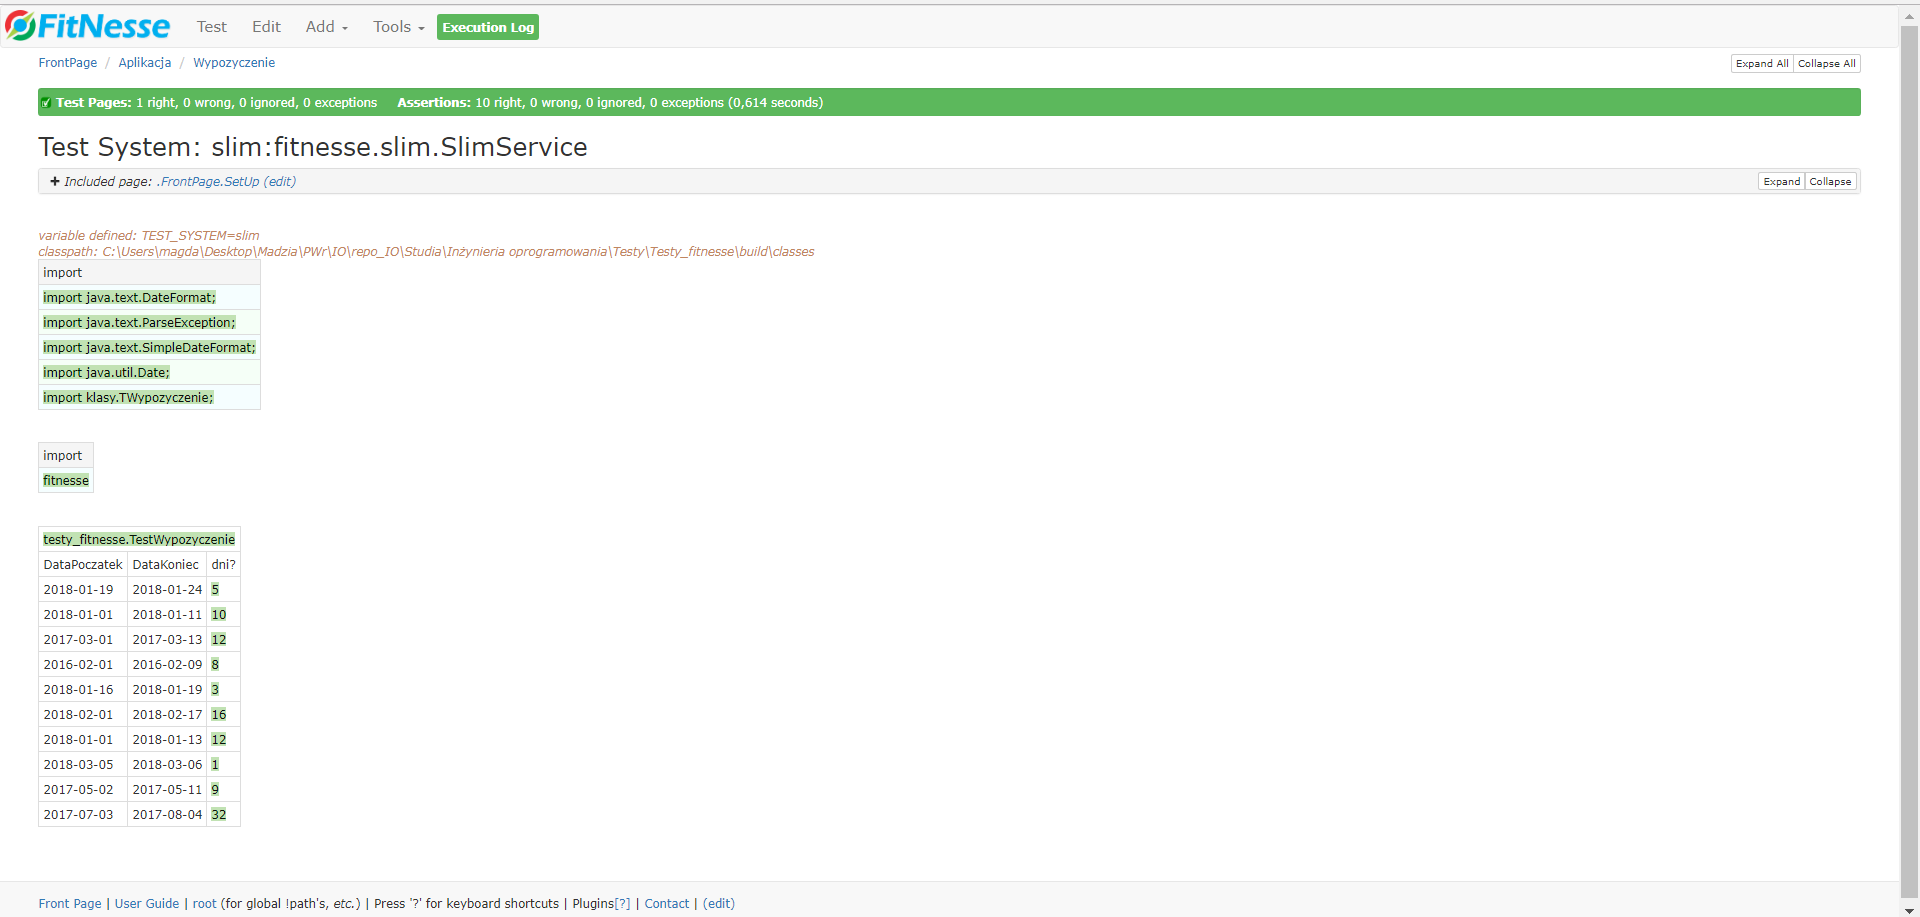
\includegraphics[width=18cm]{2.png}
	\caption{Wykonane testy}
	\label{fig:obrazek 1}
	\newpage
\end{figure}
\subsection{Testy w klasie TKlient}
Zawartość testów:
\begin{verbatim}
!define TEST_SYSTEM {slim}
!path C:\Users\magda\Desktop\Madzia\PWr\IO\repo_IO\Studia\Inżynieria oprogramowania\Testy
\Testy_fitnesse\build\classes
!|import|
|import java.text.ParseException;|
|import klasy.TestKlient;|
!|import|
|fitnesse|

!|testy_fitnesse.TestKlient|
|Imie|Nazwisko|imie?|nazwisko?|
|Magdalena|Kowal|Magdalena|Kowal|
|Maria|Nytru|Maria|Nytru|
|Jakub|Bulik|Jakub|Bulik|
\end{verbatim}
\newpage
Efekty testów:
	\begin{figure}[!ht]
	\centering
	
\includegraphics[width=18cm]{1.png}
	\caption{Efekty testów}
	\label{fig:obrazek 2}
	\newpage
\end{figure}
\subsection{Porównanie}
Tak wygląda wynik testów, gdzie dane zostały podane w złym formacie.
	\begin{figure}[!ht]
	\centering
	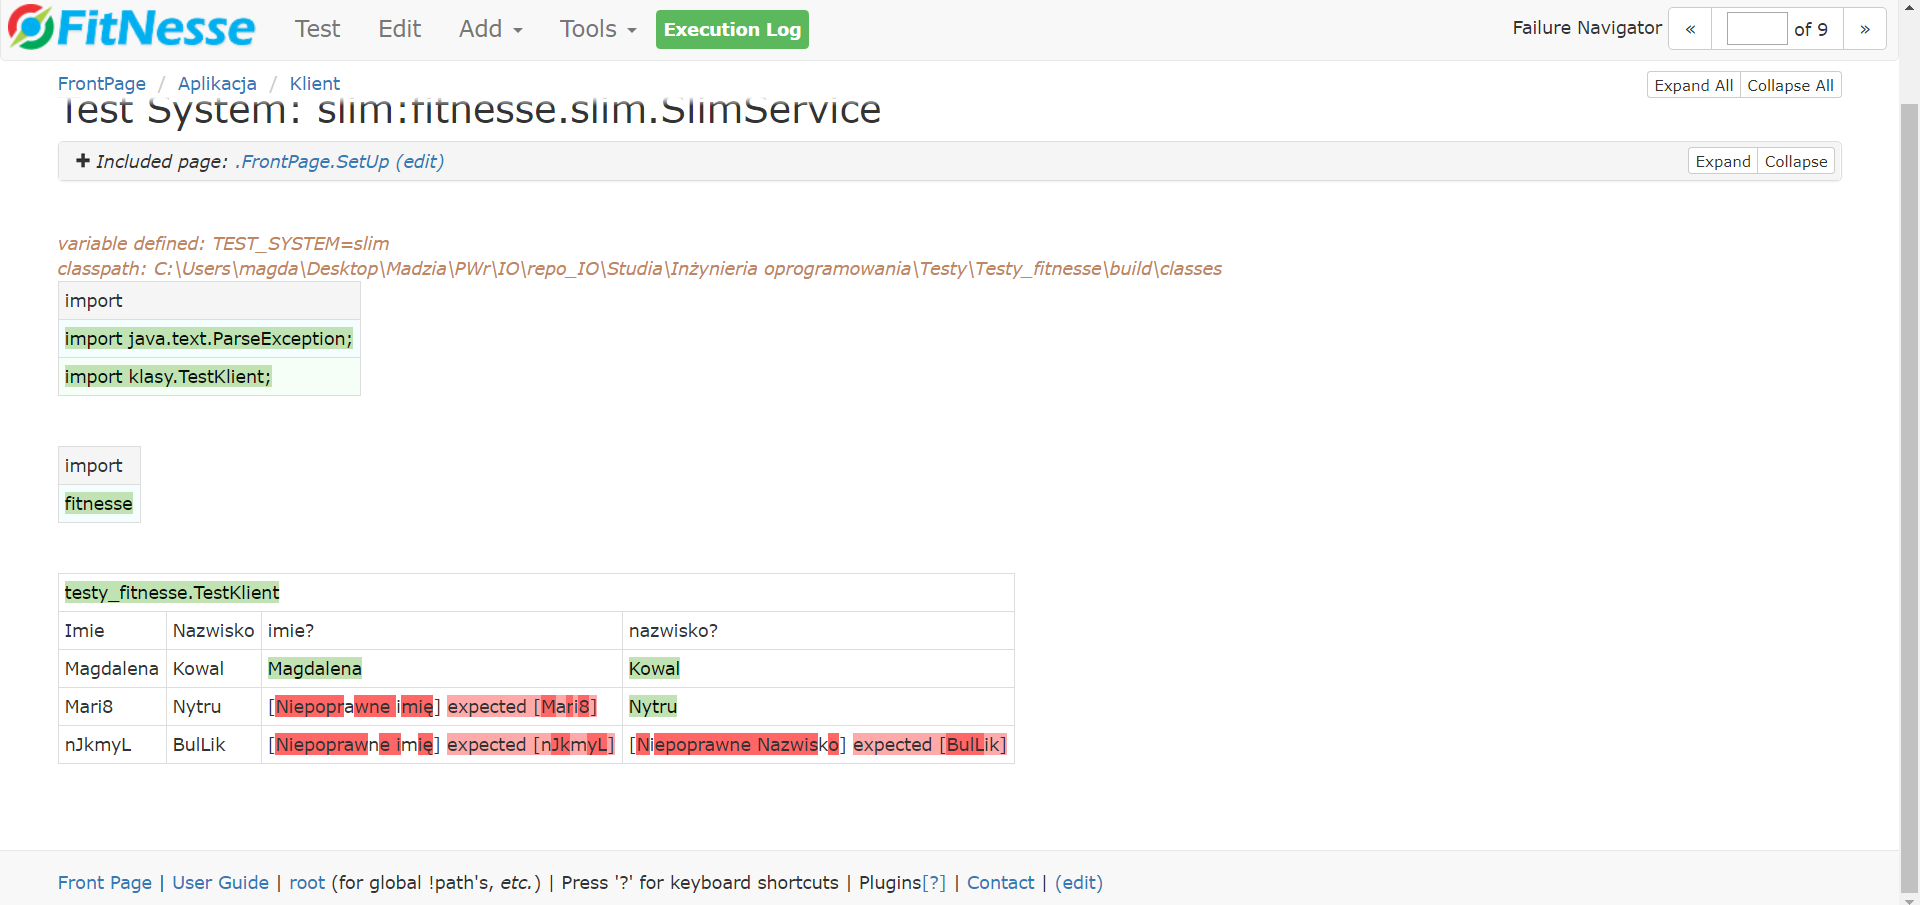
\includegraphics[width=18cm]{3.png}
	\caption{Efekty testów}
	\label{fig:obrazek 3}
	\newpage
\end{figure}
\subsection{Podsumowanie}
Testy były bardzo pouczające. Dobrze było nauczyć się je robić.
\end{document}